\documentclass[nohyperref]{article}

\usepackage{microtype}
\usepackage{graphicx}
\usepackage{subfigure}
\usepackage{booktabs}
\usepackage{amsmath}
\usepackage{amssymb}
\usepackage{mathtools}
\usepackage{amsthm}
\usepackage[UTF8,fontset=fandol]{ctex}
\usepackage{hyperref}
\usepackage[capitalize,noabbrev]{cleveref}
\usepackage[accepted]{icml2022}

\makeatletter
\renewcommand{\Notice@String}{}
\renewcommand{\printAffiliationsAndNotice}[1]{%
\stepcounter{@affiliationcounter}%
{\let\thefootnote\relax\footnotetext{\hspace*{-\footnotesep}\ifdefined\isaccepted #1\fi%
\forloop{@affilnum}{1}{\value{@affilnum} < \value{@affiliationcounter}}{
\textsuperscript{\arabic{@affilnum}}\ifcsname @affilname\the@affilnum\endcsname%
\csname @affilname\the@affilnum\endcsname%
\else
{\bf AUTHORERR: Missing \textbackslash{}icmlaffiliation.}
\fi
}.
\ \\
}%
}%
}
\makeatother

\providecommand{\theHalgorithm}{\arabic{algorithm}}
\icmltitlerunning{Beer Game RL}

\begin{document}

\twocolumn[
\icmltitle{基于强化学习的 Beer Game 库存订货控制}

\begin{icmlauthorlist}
\icmlauthor{魏知原}{pku}
\icmlauthor{孙涌畅}{pku}
\icmlauthor{首雨欣}{pku}
\end{icmlauthorlist}

\icmlaffiliation{pku}{北京大学信息科学技术学院，多智能体系统课程项目}
\icmlkeywords{Beer Game, Supply Chain, Deep Reinforcement Learning, DQN, PPO}

\vskip 0.3in
]

\printAffiliationsAndNotice{}
\chead{\small\bf Beer Game RL}

\begin{abstract}
本报告主要做的是 Beer Game 环境下的库存订货实验。我们把其中一个企业作为学习对象，尝试用几种强化学习算法来决定每一步应该订多少货。实验中先比较了一维订货动作下的 DQN、Double DQN 和 PPO，之后又把动作扩展成三维订单向量，比较 High-Dim DQN、High-Dim Double DQN 和 High-Dim PPO。单次主实验中，标准动作 PPO 的测试收益最高，为 627.90，需求满足率为 0.934；在高维动作空间中，High-Dim PPO 的测试收益为 406.63，也比另外两个高维 DQN 方法更好。由于一次实验可能受到随机性的影响，我们又对高维动作实验补充了 3 组 seed 的控制实验。在这个设置下，High-Dim PPO 的平均测试收益为 $407.18\pm21.33$，高于 High-Dim DQN 的 $339.91\pm18.37$ 和 High-Dim Double DQN 的 $306.04\pm46.72$。从这些结果看，PPO 在本项目的环境里表现相对更稳定，所以后面主要把 High-Dim PPO 作为高维订单实验的代表方法。
\end{abstract}

\section{引言}

Beer Game 是供应链管理课程中经常出现的一个例子。它的大致过程是：几个企业排成一条供应链，下游企业面对市场需求，上游企业根据下游企业的订单来补货。每个企业都要决定自己订多少货。如果订得太少，可能会缺货；如果订得太多，又会带来库存成本。因此这个问题看起来简单，但实际做决策时并不容易。

课程提供了一个基础的 Beer Game 环境，也给出了随机策略接口。本项目中，我们选择企业 $1$ 作为需要训练的智能体，其他企业用比较简单的 base-stock 策略。这样可以先把问题简化成单智能体强化学习问题。我们从 DQN baseline 做起，然后加入 Double DQN 和 PPO。除此之外，我们还把原来的一维订货量扩展成三维订单向量，想看看动作空间变复杂以后，不同算法的效果会有什么变化。

本报告把目前已经完成的实验结果放在一起比较。我们主要关心三个问题：第一，在普通的一维动作空间里，哪个算法效果更好；第二，把动作改成三维向量以后，学习难度是不是会变大；第三，在高维动作空间中，PPO 是否比 DQN 类方法更适合这个任务。

\section{环境与任务}

实验环境中一共有 $N=3$ 个企业。企业 $0$ 直接面对外部市场需求，企业 $1$ 是本项目训练的学习企业，企业 $2$ 是上游企业。每个 episode 长度为 100 步。外部需求服从泊松分布：
\begin{equation}
D_t \sim \operatorname{Poisson}(10).
\end{equation}

每个企业能看到的状态比较简单，主要包括订单量、已经满足的需求量和当前库存：
\begin{equation}
s_{i,t}=[q_{i,t}, d_{i,t}, I_{i,t}].
\end{equation}
库存的变化按照下面的公式计算：
\begin{equation}
I_{i,t+1}=I_{i,t}+q_{i,t}-d_{i,t}.
\end{equation}
也就是说，当前库存加上订货量，再减去满足的需求量，就是下一步库存。

奖励函数由销售收入、采购成本、库存成本和缺货惩罚组成：
\begin{equation}
r_{i,t}=p_i d_{i,t}-p_{i+1}q_{i,t}-hI_{i,t}-c\max(0,D_{i,t}-d_{i,t}).
\end{equation}
实验中价格设置为 $[10,9,8]$，库存持有成本 $h=0.5$，缺货惩罚 $c=2.0$，初始库存为 100。这个奖励函数的意思是，企业既要多卖货，也要控制订货和库存成本。

\section{算法与动作空间}

\subsection{标准动作算法}

在标准动作空间中，学习企业每一步只需要选择一个订货量，即 $a_t\in\{1,\ldots,20\}$。DQN 的做法是用神经网络估计每个动作的 Q 值，然后选择看起来收益比较高的动作。Double DQN 和 DQN 比较接近，只是在计算目标 Q 值时把动作选择和动作评估分开，希望减少 DQN 中可能出现的过估计问题。PPO 的思路不太一样，它直接学习一个随机策略，也就是给每个动作一个概率，再根据采样到的动作进行更新。本项目中 PPO 使用 actor-critic 网络、GAE 和 clipped objective，学习率为 $10^{-4}$，clip range 为 0.15，entropy coefficient 为 0.03，reward scaling 为 0.01。

\subsection{高维动作算法}

为了让订货动作稍微复杂一些，我们把一维订货量改成三维订单向量。每个通道可以选择 $\{0,5,10,15,20\}$ 中的一个值，同时要求三个通道的总订货量在 5 到 20 之间。去掉不满足条件的组合之后，一共有 34 个合法动作。环境中还给三个通道设置了不同的成本系数 $[1.0,1.1,1.25]$，所以智能体不仅要决定订多少，还要决定从哪个通道订。

在实现上，High-Dim DQN 和 High-Dim Double DQN 仍然是对每个离散动作学习 Q 值，只不过动作从原来 20 个标量变成了 34 个向量组合。High-Dim PPO 则把这 34 个组合作为分类策略的类别，先采样一个类别，再把它转换回具体的三维订单向量。

这种做法实现起来比较直接，也方便和 DQN 对齐。不过它也有明显缺点：比如 $(5,5,0)$ 和 $(5,0,5)$ 其实很相似，但在模型看来只是两个普通的类别，没有直接体现出它们之间的关系。所以高维动作实验的难度会更大一些，算法需要在更多组合动作中找到合适的订货方式。

\section{实验设计}

所有实验使用 Hydra 配置，输出保存在 \path{results/<algorithm>/<timestamp>/} 下，包括模型、训练分数、测试分数、测试轨迹和 \path{summary.json}。单次主实验使用当前仓库中最新可用的运行结果。标准 DQN、Double DQN、PPO，以及高维 DQN、高维 Double DQN、高维 PPO 都训练 2000 个 episode，并测试 20 个 episode。

不过，只看一次运行可能不太稳。不同算法使用的 seed offset 不完全一样，而且训练过程中消耗随机数的方式也不同，所以测试时遇到的需求序列可能不完全一致。为了让高维动作实验的比较更公平，我们又做了一个控制实验：对 High-Dim DQN、High-Dim Double DQN 和 High-Dim PPO 使用相同的 seed offset $\{0,100,200\}$，每组训练 2000 个 episode，并在测试前重置评估随机流。这样同一个 seed 下，不同算法面对的是相同的测试需求序列。

\section{单次主实验结果}

\begin{table}[t]
\caption{标准一维动作空间下 20 个测试 episode 的结果。}
\label{tab:standard}
\vskip 0.15in
\begin{center}
\begin{small}
\begin{tabular}{lccc}
\toprule
指标 & DQN & Double DQN & PPO \\
\midrule
平均收益 & 611.68 & 611.88 & \textbf{627.90} \\
收益标准差 & 60.96 & 48.61 & \textbf{39.30} \\
平均库存 & 18.04 & \textbf{16.69} & 17.41 \\
平均订货量 & 8.63 & \textbf{8.20} & 8.45 \\
需求满足率 & \textbf{0.937} & 0.917 & 0.934 \\
\bottomrule
\end{tabular}
\end{small}
\end{center}
\vskip -0.1in
\end{table}

\begin{table}[t]
\caption{三维订单向量动作空间下 20 个测试 episode 的结果。}
\label{tab:highdim-single}
\vskip 0.15in
\begin{center}
\begin{small}
\begin{tabular}{lccc}
\toprule
指标 & HD DQN & HD Double DQN & HD PPO \\
\midrule
平均收益 & 357.75 & 299.50 & \textbf{406.63} \\
收益标准差 & 100.91 & 104.83 & \textbf{74.12} \\
平均库存 & 21.73 & \textbf{20.54} & 21.51 \\
平均订货量 & 8.43 & \textbf{8.06} & 8.42 \\
需求满足率 & 0.917 & 0.904 & \textbf{0.930} \\
\bottomrule
\end{tabular}
\end{small}
\end{center}
\vskip -0.1in
\end{table}

从 \cref{tab:standard} 可以看到，在标准动作空间里，三个算法的平均收益其实差距不算特别大，但 PPO 最高，为 627.90，而且收益标准差最低。DQN 的需求满足率最高，达到 0.937，不过它的平均收益没有 PPO 高。这说明在这个环境里，并不是满足越多需求就一定收益越高，因为多订货也会带来采购成本和库存成本。Double DQN 的结果和 DQN 很接近，平均收益只略高一点，但方差更低。

\cref{tab:highdim-single} 是高维动作空间的结果。可以看出，高维动作下所有方法的收益都比标准动作低，说明三维订单向量确实让问题变难了。在三种高维方法中，High-Dim PPO 的平均收益最高，为 406.63，而且标准差最小。High-Dim DQN 的收益为 357.75，High-Dim Double DQN 只有 299.50。从这个结果看，PPO 在高维动作空间里表现得更稳定一些。

\begin{figure}[t]
\vskip 0.1in
\begin{center}
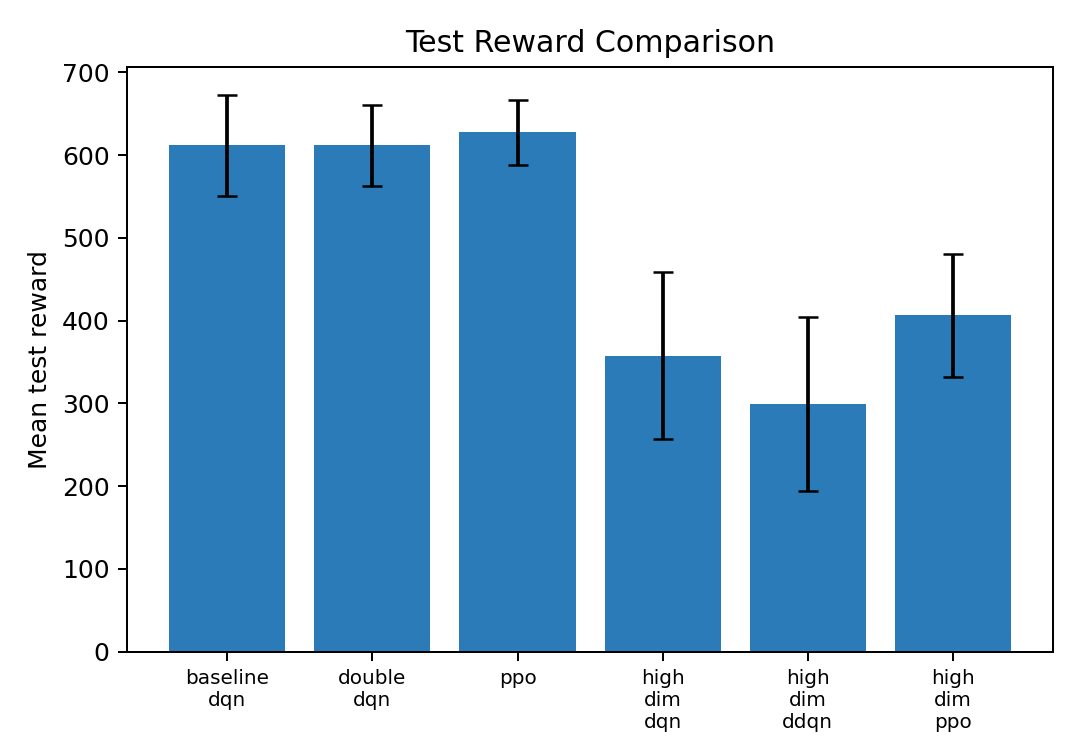
\includegraphics[width=\columnwidth]{images/summary_205932_comparison_test_scores.png}
\caption{单次主实验的测试收益对比。}
\label{fig:single-test}
\end{center}
\vskip -0.15in
\end{figure}

\begin{figure}[t]
\vskip 0.1in
\begin{center}
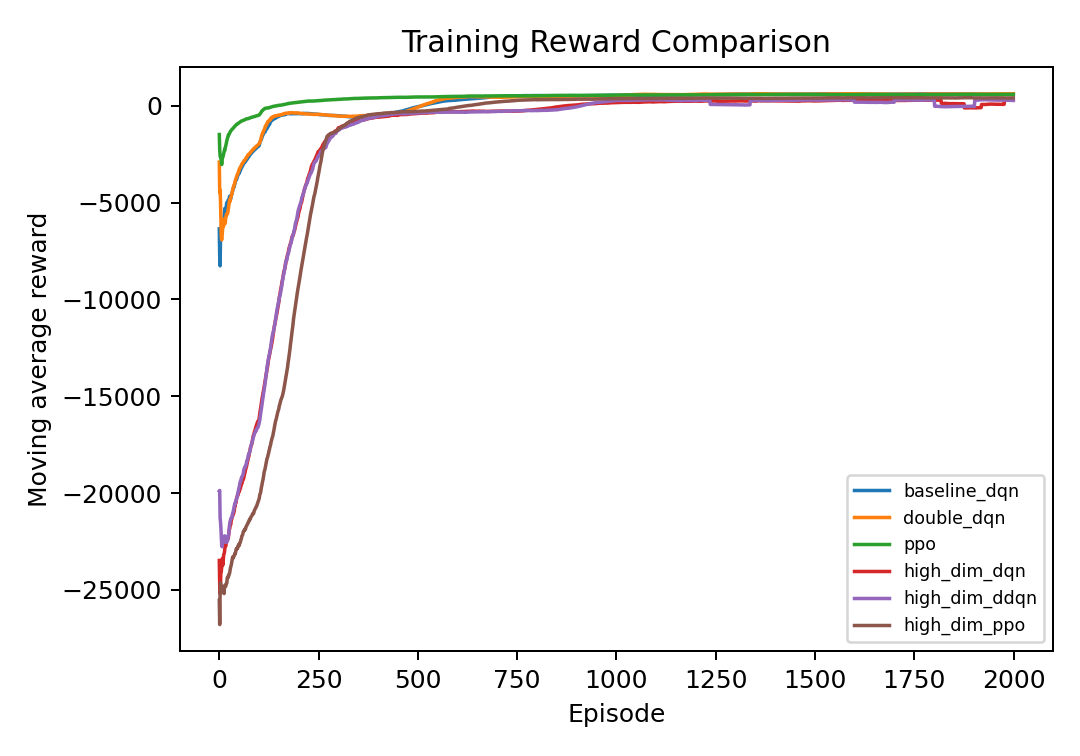
\includegraphics[width=\columnwidth]{images/summary_205932_comparison_training_curve.png}
\caption{单次主实验的训练收益移动平均曲线。}
\label{fig:single-training}
\end{center}
\vskip -0.15in
\end{figure}

\cref{fig:single-test} 中也能看到类似结论：标准动作空间下 PPO 的测试收益最高，高维动作空间中也是 High-Dim PPO 更好。\cref{fig:single-training} 展示了训练过程。相比标准动作方法，高维动作方法在训练初期的收益更低，波动也更明显，这和动作空间变复杂是符合预期的。

\section{控制实验结果}

\begin{table}[H]
\caption{高维动作控制实验。均值和标准差按 3 个训练 seed 统计；每个 seed 的测试均值来自 20 个 episode。}
\label{tab:controlled}
\vskip 0.15in
\begin{center}
\begin{small}
\begin{tabular}{lcccc}
\toprule
方法 & 平均收益 & 满足率 & 库存 & 订货 \\
\midrule
HD PPO & \textbf{407.18$\pm$21.33} & \textbf{0.946} & \textbf{22.25} & 8.43 \\
HD DQN & 339.91$\pm$18.37 & 0.934 & 22.76 & \textbf{8.32} \\
HD Double DQN & 306.04$\pm$46.72 & 0.938 & 23.07 & 8.35 \\
\bottomrule
\end{tabular}
\end{small}
\end{center}
\vskip -0.1in
\end{table}

\begin{figure}[H]
\vskip 0.02in
\begin{center}
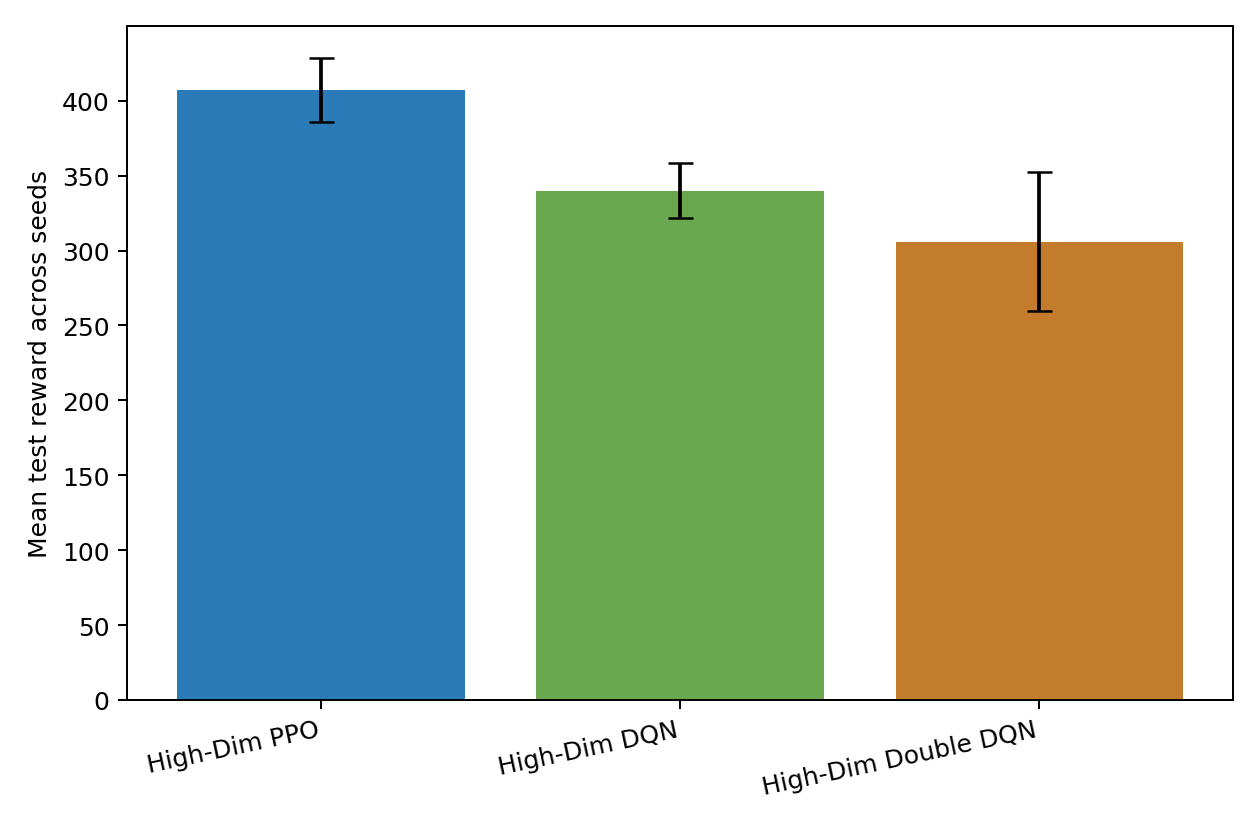
\includegraphics[width=0.88\columnwidth]{images/controlled_high_dim_main_rewards.png}
\caption{高维动作 3-seed 控制实验的平均测试收益。}
\label{fig:controlled}
\end{center}
\vskip -0.12in
\end{figure}

为了进一步确认高维动作下的结果，我们做了 3 个 seed 的控制实验。\cref{tab:controlled} 和 \cref{fig:controlled} 中，High-Dim PPO 的平均收益为 $407.18\pm21.33$，仍然高于 High-Dim DQN 和 High-Dim Double DQN。High-Dim DQN 的平均收益为 $339.91\pm18.37$，High-Dim Double DQN 为 $306.04\pm46.72$。可以看到，Double DQN 在这里并没有带来提升，反而波动更大。表现最好的一次 High-Dim PPO 来自 seed offset 200，测试均值达到 424.95，需求满足率为 0.949。因此我们把这组结果作为高维动作实验中比较有代表性的结果。

\section{讨论}

从实验结果看，标准一维动作策略的收益仍然比高维动作策略更高。这个结果一开始有点出乎预期，因为高维动作看起来表达能力更强，可以选择不同通道的订货组合。但后来分析后发现，当前实现只是把所有合法向量枚举成 34 个类别，模型并不知道这些动作之间有什么联系。因此动作变多以后，学习难度也变大了。

在高维动作实验中，PPO 的表现相对最好。一个可能原因是 PPO 本身是随机策略，并且使用了熵正则，所以训练过程中会持续探索不同的订单组合。而 DQN 类方法主要依赖 Q 值估计，如果动作数量变多，Q 值估计的噪声可能会影响动作选择。尤其是 High-Dim Double DQN，在本实验中没有比 High-Dim DQN 更好，说明 Double DQN 的改进在这个设置下不一定总是有效。

标准动作实验还说明，收益和需求满足率不是完全一致的指标。比如 DQN 的需求满足率略高于 PPO，但平均收益反而低一些。这说明库存控制不能只看是否满足需求，还要同时考虑采购成本和库存成本。如果后续继续改进高维动作方法，可能需要让模型更好地利用订单通道之间的结构，比如让策略分别决定每个通道的订货量，而不是直接在 34 个完整组合中选择。

\section{结论}

本项目比较了 Beer Game 环境下几种强化学习订货策略。实验结果显示，在标准一维动作空间中，PPO 的平均收益最高，收益波动也最小。在三维订单向量的高维动作空间中，High-Dim PPO 也比 High-Dim DQN 和 High-Dim Double DQN 表现更好。虽然高维动作空间理论上提供了更灵活的订货方式，但当前简单枚举动作的实现会增加学习难度，因此总体收益低于标准动作实验。综合来看，PPO 是本项目中比较合适的方法，后续如果继续做，可以重点改进高维动作空间的建模方式。

\end{document}
